\chapter{Détection des événements extrêmes}

Au-delà de la performance moyenne en régression, il est utile d'évaluer la capacité du modèle à détecter les fortes variations de production, appelées ici rampes critiques. Cette analyse transforme temporairement le problème de régression en problème de détection binaire.

Un seuil Q90 est défini à partir de l'ensemble de développement. Les observations dont la variabilité est supérieure ou égale à ce seuil sont considérées comme critiques. Dans le notebook, le seuil obtenu est : $Q90 = 8.04$

La même logique est appliquée aux prédictions du modèle : si la variabilité prédite dépasse le seuil retenu, le modèle déclenche une alerte de rampe critique.

\section{Résultats avec le seuil Q90}


\begin{figure}[htbp]
    \centering
    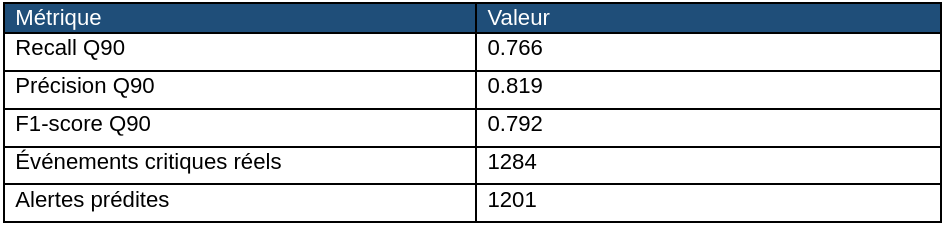
\includegraphics[width=0.9\textwidth]{img/tab_8_1.png}
    \caption{Résultats de détection des rampes critiques avec le seuil Q90.}
    \label{fig:tab_8_1}
\end{figure}

\begin{figure}[htbp]
    \centering
    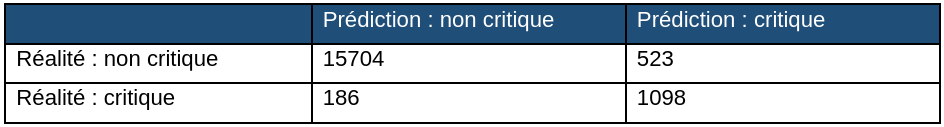
\includegraphics[width=0.9\textwidth]{img/tab_8_4.png}
    \caption{Matrice de confusion avec le seuil Q90.}
    \label{fig:tab_8_4}
\end{figure}


Avec le seuil Q90, le modèle détecte correctement 984 événements critiques parmi les 1284 réellement présents dans l'ensemble de test. Il manque donc 300 rampes critiques, soit environ 23.4 % des événements critiques.

En parallèle, le modèle produit 217 fausses alertes sur 16 227 situations non critiques. La précision atteint donc environ 81.9 \%, ce qui signifie que les alertes émises sont généralement fiables. Le recall de 76.6 % indique que le modèle identifie une grande partie des événements extrêmes, mais qu'une partie des rampes critiques reste non détectée.

Dans ce contexte, l'accuracy globale doit être interprétée avec prudence, car les événements critiques sont minoritaires. Les métriques les plus pertinentes sont donc le recall, la précision et le F1-score de la classe critique.

\section{Ajustement du seuil de décision}

Dans une application opérationnelle, le seuil utilisé pour définir les événements critiques réels peut être différent du seuil de décision appliqué aux prédictions. En abaissant le seuil de décision, le modèle devient plus sensible : il détecte davantage de rampes critiques, mais il génère aussi davantage de fausses alertes.

Le notebook teste plusieurs seuils et sélectionne un seuil permettant d'obtenir au moins 85 \% de recall tout en maximisant la précision. Le seuil optimisé obtenu est 7.372.

\begin{figure}[htbp]
    \centering
    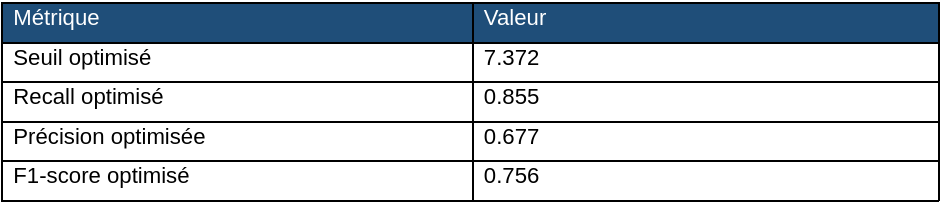
\includegraphics[width=0.9\textwidth]{img/tab_8_3.png}
    \caption{Résultats avec le seuil de décision optimisé.}
    \label{fig:tab_8_3}
\end{figure}

\begin{figure}[htbp]
    \centering
    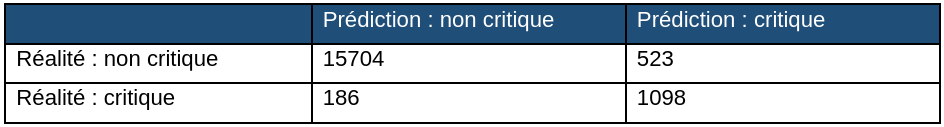
\includegraphics[width=0.9\textwidth]{img/tab_8_4.png}
    \caption{Matrice de confusion avec le seuil optimisé.}
    \label{fig:tab_8_4}
\end{figure}


Avec le seuil optimisé, le modèle détecte correctement 1098 événements critiques parmi les 1284 présents dans l'ensemble de test. Le recall atteint environ 85.5 \%, ce qui signifie que le modèle manque seulement 186 rampes critiques, soit environ 14.5 \% des événements critiques.

En contrepartie, le nombre de fausses alertes augmente de 217 à 523, et la précision diminue à environ 67.7 \%. Ce résultat traduit un compromis orienté vers une meilleure détection des événements extrêmes plutôt que vers une précision maximale des alertes.

Comparé au seuil Q90, le seuil optimisé améliore nettement la capacité de détection : le recall passe de 76.6 \% à 85.5 \%. Le choix final du seuil dépend donc du coût opérationnel relatif entre une rampe critique manquée et une fausse alerte.
